\documentclass{article}
\usepackage{geometry}
\usepackage{url}
\usepackage[utopia]{mathdesign}
\geometry{
  a4paper,
  total={170mm,257mm},
  left=20mm,
  top=20mm,
}
\usepackage{graphicx}
\usepackage{titling}

\title{Report for soft end effectors}
\author{GU JUN}
\date{Jan 15th, 2025}

\usepackage{fancyhdr}
\setlength{\headheight}{12.49998pt}
\addtolength{\topmargin}{-0.49998pt}
\fancypagestyle{plain}{%  the preset of fancyhdr 
    \fancyhf{} % clear all header and footer fields
    \fancyfoot[R]{\thepage}
    \fancyfoot[L]{\thedate}
    \fancyhead[L]{Soft Robotics Home Assignment \#7}
    \fancyhead[R]{\theauthor}
}
\makeatletter
\renewcommand{\maketitle}{%
  \newpage
  \null
  \vskip 1em%
  \begin{center}%
  \let \footnote \thanks
    {\LARGE \@title \par}%
    \vskip 1em%
    %{\large \@date}%
  \end{center}%
  \par
  \vskip 1em}
\makeatother

\usepackage{lipsum}  
\usepackage{cmbright}

\begin{document}

\maketitle

\noindent\begin{tabular}{@{}ll}
    Student & \theauthor\\
    Date & \thedate\\
    Assignment & Soft Robotics Home Assignment \#6\\
\end{tabular}\\

% 1. Think of one target object that is difficult to handle by conventional EEs;

% 2. Write down the reason why it is difficult to grasp;

% 3. Propose a soft robotic EE that can handle the object at high-speed;

% 4. If possible, make a CAD design and insert the drawing; at least make a handwritten sketch;

\section*{Problem statement - Difficult object to handle}
In japan, there is a traditional game called "Kingyo Sukui" which is to catch golden fishes with a paper scoop. 
The game is very hard for humans, and it is also difficult for robots.
Golden fishes are difficult to handle by conventional end effectors (EEs) due to their soft and slippery body. 
The conventional EEs are designed to handle rigid objects, and they are not suitable for handling soft objects, especially living creatures. 
\begin{figure}[h!]
    \centering
    \includegraphics[width=0.3\textwidth]{assets/golden_fishes.pdf}
    \caption{Travelers are playing "Kingyo Sukui" in Japan.}
\end{figure}
Here are the reasons why golden fishes are difficult to grasp:
\begin{itemize}
    \item Slippery and soft body: Golden fishes have a protective mucus layer on their body, which makes them slippery.
    \item Living creatures: Golden fishes are living creatures with high mobility, sensitivity, and active behaviors.
    \item Fragile: Golden fishes are fragile, which mean the robotic EE should handle them gently to avoid hurting them.
\end{itemize}
\section*{Proposed solution - A net-like soft robotic EE}
Inspired by the soft end effector in the lecture, I propose a net-like soft robotic EE to handle the golden fishes.
\begin{figure}
    \centering
    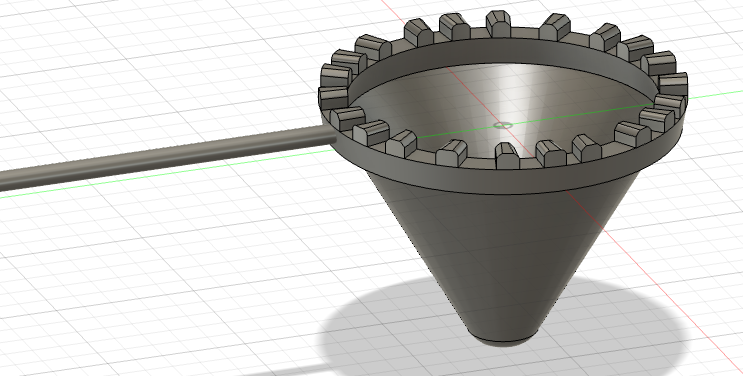
\includegraphics[width=0.3\textwidth]{assets/net_ee.png}
    \caption{\textbf{CAD design of the net-like soft robotic EE.} The net-like soft robotic EE is made by 3 parts, a net, a soft actuator, and a handle with an air pipe.}
\end{figure}

The net-like soft robotics EE is made by 3 parts, a handle with an air pipe, a soft actuator, and a net. The soft actuator is on the net to open/close the net.
The net is made by soft and flexible materials, which can adapt to the shape of the golden fishes.
The soft actuator is made by soft pneumatic actuators, which can provide a gentle force to open/close the net. 

\end{document}
